\documentclass[12pt,a4paper]{scrbook}
\usepackage[utf8]{inputenc}
\usepackage[ngerman]{babel}
\usepackage{amsmath}
\usepackage{amsfonts}
\usepackage{amssymb}
%~ \usepackage[left=2.5cm,right=2cm,top=3cm,bottom=2cm]{geometry}
\usepackage{graphicx}
\usepackage{relsize}
\usepackage[bottom]{footmisc}
\usepackage[hidelinks]{hyperref}
\usepackage{color}
\author{Patrick Eigensatz\\Gabriel Gavrilas}
\title{Mathematik in der Kantonsschule}

\begin{document}
\shorthandoff{"}

\maketitle
\section*{Vorwort}
Dieses Buch enstand als Zusammenfassung der ganzen Mathematik Theorie in der Kantonsschule.
Dabei wurden die Themen aus dem Grundlagenfach, wie auch die Themen aus dem Akzentfach
aufgenommen.

\makeatletter
\renewcommand*\cleardoublepage{\clearpage\if@twoside
  \ifodd\c@page \hbox{}\newpage\if@twocolumn\hbox{}%
  \newpage\fi\fi\fi}
\makeatother

\tableofcontents
\newpage

\part{1. Kantonsschule}

\chapter{Potenzgesetze}


\chapter{Strahlensätze und Ähnlichkeit}


\chapter{Funktionen}
\section{Definition einer Funktion}
Die Definition erfolgt durch eine Deklaration inklusive
der Zahlbereichen und des Zahlbereiches des "Rückgabewertes" der Funktion:

\[ f : \mathbb{R} \rightarrow \mathbb{R}\]
\[ f(x) = \frac{3}{7} + a^2 - \frac{b}{3x} + 2; \quad\quad x \in \mathbb{Z}\backslash\{0\}\]

\section{Lineare Funktion}
\subsection{Typische Definition}
\[f(x) = y = k \cdot x + d; \quad\quad k, d \in \mathbb{R}\]
\subsection{Lösungsformel}
\[x = \frac{-d}{k}\]

\subsection{Beispiel}
\[f(x) = -\frac{3}{2}x + 6\]

\subsection{Wertetabelle} der Funktion $f(x)$ wobei $x \in [-3; 7]$\\\\
\begin{tabular}{l||c|c|c|c|c|c|c|c|c|c|c}
$x$ & -3 & -2 & -1 & 0 & 1 & 2 & 3 & 4 & 5 & 6 & 7\\
\hline
$f(x)$ & 10.5 & 9 & 7.5 & 6 & 4.5 & 3 & 1.5 & 0 & -1.5 & -3 & -4.5\\
\end{tabular}\\\\\\
\textbf{Beachte:} $\Delta x$ ist konstant $-1.5$.\\

\subsection{Steigung}
\[f(x) = k\cdot x + d; \quad\quad k,d \in \mathbb{R}\]
$d$ ist der y-Achsenabschnitt. An diesem Ort wird die y-Achse\\
geschnitten. $k$ ist die Steigung von f.\\\\\\
\begin{tabular}{ll}
Wenn $k \geq 0$: & f ist wachsend\\
Wenn $k < 0$: & f ist fallend\\
\end{tabular}

\subsection{Stufenformel}
Herleitung der Stufenformel:
\[f(x+1) = f(x) + k\]
\[f(x+1) - f(x) = k\]
\[f(x+\Delta x) = f(x) + \Delta x \cdot k\]
\[f(x+\Delta x) - f(x) = \Delta x \cdot k\]
\[f(x+\Delta x) - f(x) = k\]

\begin{center}
\fbox{\parbox{4cm}{\[\frac{\Delta y}{\Delta x} = k\]}}
\end{center}


\subsubsection{Deutung der Steigung k}
Die Steigung einer linearen Funktion entspricht der Änderung\\
der Funktionswerte, bei Vermehrung des Arguments um 1.

\section{Quadratische Funktion}
\subsection{Typische Definition}
\[f(x) = y = ax^2 + bx + c; \quad\quad a \in \mathbb{R}\backslash\{0\}; \;\; b, c \in \mathbb{R}\]
\subsection{Lösungsformel}
\[x_1 / x_2 = \frac{-b \pm \sqrt{b^2-4ac}}{2a} \]
\subsection{Beispiel}
\[f(x) = \frac{1}{2}x^2 - \frac{3}{4}x - \frac{7}{2}\]

\subsection{Wertetabelle} der Funktion $f(x)$ wobei $x \in [-3; 7]$\\\\
\begin{tabular}{l||c|c|c|c|c|c|c|c|c|c|c}
$x$ & -3 & -2 & -1 & 0 & 1 & 2 & 3 & 4 & 5 & 6 & 7\\
\hline
$f(x)$ & 3.25 & 0 & -2.25 & -3.5 & -3.75 & -3 & -1.25 & 1.5 & 5.25 & 10 & 15.75\\
\end{tabular}\\\\\\
\textbf{Beachte:} $\Delta x$ ist nicht konstant!\\


\chapter{Quadratische Gleichungen}
\label{quadratische_gleichungen}


\chapter{Lineare Gleichungssysteme}

\chapter{Trigonometrie}

\chapter{Logik}
\section{Aussagen}
\section{Logikoperatoren}

\chapter{Mengen}
\section{Mengenoperationen}

\chapter{Beweise}
\section{Direkte Beweise}

\section{Indirekte Beweise}

\section{Induktive Beweise}

\chapter{Darstellende Geometrie}
\section{Einführung}
\textbf{Grundproblem:} räumliche Figur $\Leftrightarrow$ ebene Zeichnung \\\\
Die Darstellende Geometrie schafft Grundlagen für die zeichnerische, ebene Darstellung räumlicher Objekte
und die zeichnerische Lösung räumlicher Probleme. In der Mathematik sind die
folgenden Abbildungsverfahren gebräuchlich:

\begin{itemize}
  \item Schrägbild
  \item Darstellung mit einem oder mehreren Rissen
\end{itemize}

\begin{figure}[h]
  \centering
  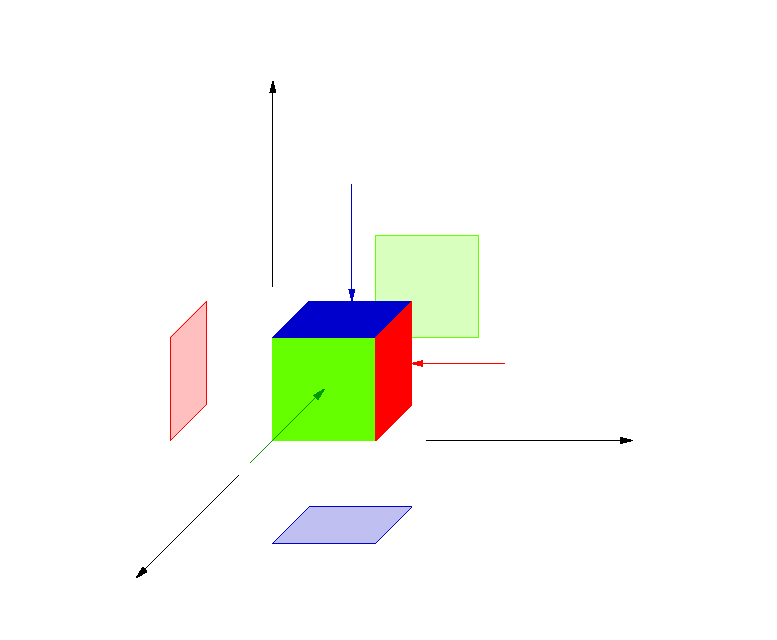
\includegraphics[scale=1]{img/DGeinfuehrung.pdf}
  \caption{Die verschiedenen Risse}
  \textcolor{blue}{Grundriss (Vogelperspektive)}\\
  \textcolor{green}{Aufriss (Ansicht von vorne)}\\
  \textcolor{red}{Seitenriss (Kreuzriss, Ansicht von der Seite)}
\end{figure}


\subsection{Kavaliersprojektion}
\begin{figure}[h]
  \centering
  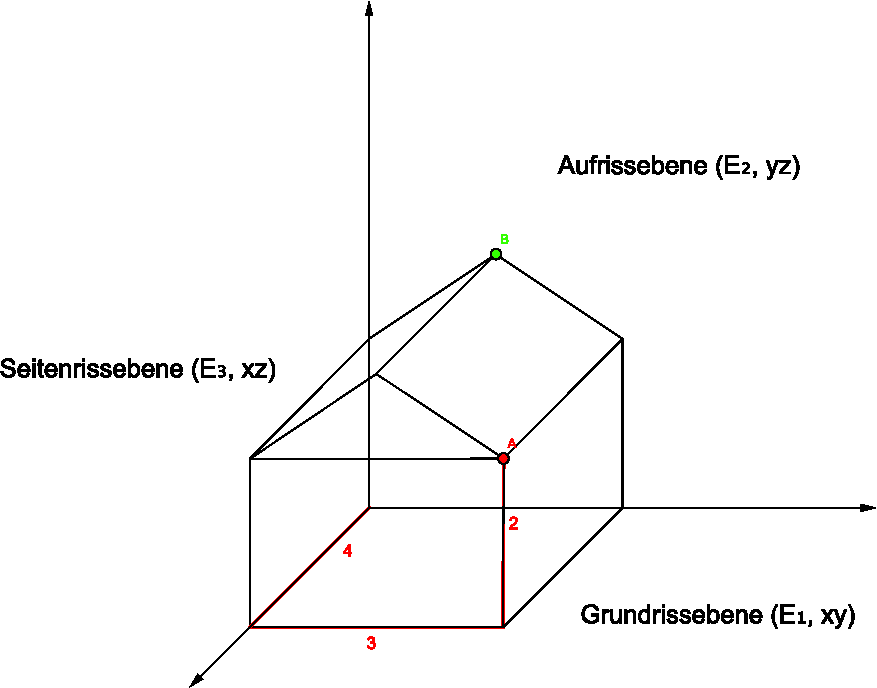
\includegraphics[scale=0.8]{img/DGeinfuehrung_2.pdf}
  \caption{Beispiel Kavaliersprojektion}
\end{figure}

\begin{enumerate}
\item $a_{xy} = 135^{\circ}$ Verzerrungswinkel
\item $k_{x} = \frac{1}{2}$ Verzerrungsfaktor
\end{enumerate}

\subsection{Dotierte Eintafeldarstellung}
(Ansicht von oben mit zusätzlicher Angabe der Höhe(nkote)
\begin{figure}

\end{figure}

\section{Kavaliersprojektion}
\section{Zweitafeldarstellung}
\section{Dreitafeldarstellung}


\chapter{Komplexe Zahlen}
\section{Grundlagen}
Während unserem ganzen Leben erweiteren wir unsere Zahlbereiche. Zuerst
reichten unsere natürlichen Zahlen von 0 bis 10. Irgendwann kamen die Zahlen,
die grösser als 10 sind dazu ($\mathbb{N}$). Später entdeckten wir
negative Zahlen ($\mathbb{Z}^-$). Es kamen die rationalen Zahlen hinzu.
(z. Bsp. $\frac{1}{4} = 0.25 \in \mathbb{Q}$). Um alle möglichen Werte auf
der Zahlengerade bestimmen zu können (z. Bsp. $\sqrt{2} \in \mathbb{R}$)
beschrieb man die reellen Zahlen. Etwas später endeckte man, dass
gewisse Probleme nicht mehr in den reellen Zahlen lösbar sind.
Zum Beispiel einige quadratische Gleichungen:\footnote{Wie man quadratische Gleichungen lösen kann,
erfährt man auf Seite \pageref{quadratische_gleichungen}}
\begin{eqnarray*}
x^2+4 & = ~ 0\\
x^2+4x+13 & = ~ 0\\
x^2+1 & = ~ 0
\end{eqnarray*}
Deshalb wurden die komplexen Zahlen ($\mathbb{C}$) beschrieben. Die komplexen
Zahlen sind eine "Übermenge" der reellen Zahlen. Es gilt also:
\[\mathbb{N} ~ \subset ~ \mathbb{Z} ~ \subset ~ \mathbb{Q} ~ \subset ~ \mathbb{R} ~ \subset ~ \mathbb{C}\]
Das Problem in reellen Zahlen besteht darin, dass Wurzeln mit negativen
Radikanden unmöglich zu berechnen sind.
\[\sqrt{-100} ~~ (Existiert~in~\mathbb{R}~nicht)\]
Quadriert man jedoch eine negative Zahl, ist das Resultat stets positiv.\\
In den reellen Zahlen können alle Zahlen innerhalb eines Intervalles (z. Bsp.
$]3, 5]$) genannt werden. Um also Lösungen erhalten zu können, die nicht auf
einer eindimensionalen Strecke liegen, machen wir den Zahlenbereich zweidimensional.
Zahlen haben nun also 2 Koordinaten. Dies kann wie folgt geschrieben werden, wobei
letztere Schreibweise gebräuchlicher ist:
\[(4, 3i) = 4 + 3i\]
Das $i$ stellt die imaginäre Einheit dar, wobei gilt, dass:
\begin{center}
\fbox{\parbox{4cm}{\[i^2 = -1\]}}
\end{center}
Da die komplexen Zahlen aus einem Real- und einem Imaginärteil bestehen, ist es auch nicht mehr möglich,
diese in Relationen zu einander zu setzen. ($<, \leq, ...$)

\section{Konjugiert komplexer Wert}
Der konjugiert komplexe Wert einer komplexen Zahl entspricht der Zahl selbst,
mit der Ausnahme, dass das Vorzeichen des imaginären Wertes geändert wurde. Formell:
\[\overline{(a+bi)} = \left\lbrace \begin{array}{ll} (a-bi), & wenn~b > 0\\ (a+bi), & sonst \end{array} \right.\]
Ein konkretes Beispiel:
\[\overline{(4+3i)} = (4-3i)\]

\section{Kartesische Darstellung}
Da wir auf unserem eindimensionalen Zahlenstrahl bereits alle Werte
beschreiben können, erweitern wir den Strahl auf eine zweidimensionale
Ebene. Die x-Achse wird als die "reelle Achse" bezeichnet, wohingegen,
die neue hinzugekommene y-Achse "imaginäre Achse" genannt wird.\\
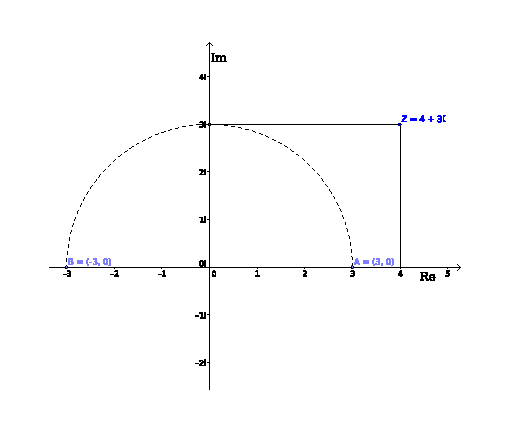
\includegraphics[scale=1.9]{img/komplexe_zahlen.pdf}

\section{Polardarstellung}
In der Polardarstellung wird die Zahl nicht durch Koordinaten auf der x- und der y-Achse angegeben, sondern
durch den Abstand vom Nullpunkt\footnote{Siehe auch die Betragsfunktion: Seite \pageref{komplex_betrag}}
\[r = \vert z \vert = \sqrt{Re(z)^2 + Im(z)^2} \]
und den Öffnungswinkel $\phi$. Für die Polardarstellung haben sich folgende Schreibweisen eingebürgert:
\[(\sqrt{2}, 45^{\circ}) = \sqrt{2} ~~ cis ~~ 45^{\circ} = 1 + i\]
Das $cis$ steht hierbei für $\cos$, $i$ und $\sin$, die trigonometrischen Funktionen, die bei der Berechnung mit Polarkoordinaten gebraucht werden. Auf diese Berechnungen wird hier nicht weiter eingegangen.\\
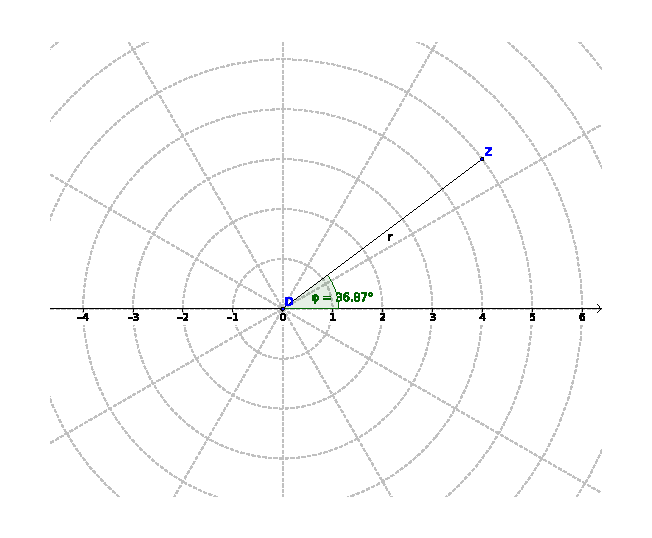
\includegraphics[scale=1.5]{img/komplexe_zahlen_polar.pdf}\\

\section{Rechenoperationen}
Bei den Grundrechenarten könnte man $i$ als Formvariable betrachten, mit der ganz normal gerechnet wird, wobei zu beachten ist, dass ein $i^2$ durch ein $-1$ zu
ersetzen ist.
\subsection{Addition}
Die Addition zweier komplexer Zahlen gestaltet sich ganz einfach.
Es müssen nur jeweils die Realteile und die Imaginärteile zusammengezählt werden. Beispiel:
\[(4+3i) + (2+2i) = (6+5i)\]

\subsection{Subtraktion}
Die Subtraktion erfolgt analog zur Addition:
\[(2+2i) - (4+3i) = (-2-1i)\]

\subsection{Multiplikation}
Auch bei der Multiplikation, wird ganz normal jeder Summand mit jedem multipliziert.
Wichtig zu wissen ist hier, dass $i^2 = -1$ definiert wurde.
\begin{equation*}
\begin{split}
(4+3i) \cdot (2+2i) & = 8 + 8i + 6i + 6i^2 \\
 & = 8 + 14i + 6(-1)\\
 & = 2 + 14i
\end{split}
\end{equation*}

\subsection{Division}
Bei der Division (vereinfacht meist als Bruch), müssen Zähler und Nenner mit
dem konjugiert komplexen Wert des Nenners erweitert werden:
\[\frac{z_1}{z_2} = \frac{z_1 \cdot \overline{z_2}}{z_2 \cdot \overline{z_2}}\]
Dies ist notwendig, um ein $i^2$ zu generieren und somit die Imaginärteile aus dem
Nenner kürzen. Im Nenner ergibt sich dadurch ein Binom. Beispiel:
\[
\frac{(4+3i)}{(2+2i)} ~ = ~ \frac{(4+3i)(2-2i)}{(2+2i)(2-2i)}
~ = ~ \frac{8-2i-6i^2}{4-4i^2} ~ = ~ \frac{14-2i}{8} ~ = ~ \frac{7}{4} - \frac{1}{4}i
\]

\subsection{Betrag}
\label{komplex_betrag}
Der Betrag einer komplexen Zahl entspricht dem Abstand zum Nullpunkt auf der
Gaussschen Ebene.
\[r = \vert z \vert = \sqrt{Re(z)^2 + Im(z)^2} \]

\section{Quadratische Gleichungen}
Quadratische Gleichungen mit komplexen Lösungen lösen sich mit derselben
Lösungsformel wie quadratische Gleichungen mit reellen Lösungen.\footnote{Siehe Seite \pageref{quadratische_gleichungen}}
\[z^2 + 4z + 5 = 0\]
\[\Rightarrow z_{1/2} = \frac{-4 \pm \sqrt{16-20}}{2} \]
Reelle Lösungen lassen sich durch die Diskriminate ausschliessen:
\[16-20 < 0 ~ \Longrightarrow ~ \sqrt{-4} = 2i\]
\[\frac{-4 \pm 2i}{2} = -2 \pm i\]
Hat man eine Lösung einer quadratischen Gleichung, erhält man die 2. Lösung durch
den konjugiert komplexen Wert der 1. Lösung:
\[z_2 = \overline{z_1}\] 


\chapter{Beschreibende Statistik}
\section{Einführung}
Bei der beschreibenden Statistik geht es grundsätzlich um die Darstellung von Daten.
Bevor man Daten auswerten kann, werden diese meist erhoben. (Leute werden befragt, etc.)
Die Daten beziehen sich meistens nur auf eine gewisse Menge innerhalb der Grundmenge.
Es werden nie alle Leute zu einem Thema befragt, jedoch einzelne an vielen Orten.

\section{Variablenwerte}
Erhoben werden dabei Variablenwerte (Merkmalsausprägungen), die Variabeln (Merkmalen) zugeordnet werden.
Beispiele:\\\\
\begin{tabular}{|ll|}
Augenfarbe & blau, braun,  grün, grau\\
Mathematiknote & 1, 2, 3, 4, 5, 6\\
Körpergrösse & 150cm, 160cm, 170cm, ...
\end{tabular}

\section{Variabeltypen}
\begin{description}
  \item[Nominale oder qualitative Variable] Diese Variabeln dienen jediglich zur Unterscheidung. Zum Beispiel: Geschlecht, ja/nein, etc.
  \item[Ordinale Variable] Zwischen diesen Variablen besteht eine Rangordnung, die Abstände sind nicht immer gleich. Zum Beispiel: Schulnote, Ranglistenplatz, etc.
  \item[Metrische Variable] Zwischen diesen Variablen sind die Abstände vergleichbar. Zum Beispiel: Körpergrösse, Gewicht.
\end{description}

\section{Die Urliste}
In der Urliste befinden sich die Rohdaten, also noch nicht ausgewertet, aber chronologisch, nach Eingabe der Daten geordnet.

\section{Visualisierungen}
\subsection{Säulendiagramm}
\subsection{Histogramm}
\subsection{Kreisdiagramm}
\subsection{Boxplot}

\section{Spezielle Werte}
\subsection{Das arithmetische Mittel}
\subsection{Der Median}
\subsection{Quartile}
Interquartilsabstand

\subsection{Der Modus}
\subsection{Empirische Varianz}
\[ s^2 = \sigma^2_x = \frac{(x_1-\overline{x})^2 + (x_2-\overline{x})^2 + ... + (x_n-\overline{x})^2}{n} = \sum_{i=1}^n \frac{(x_i-\overline{x})^2}{n} = \frac{1}{n}\sum_{i=1}^n (x_i-\overline{x})^2\]

\subsection{Standardabweichung}
\[ s_x = \sigma_x = \sqrt{\sigma^2_x} = \sqrt{\frac{1}{n} \sum_{i=1}^n (x_i-\overline{x})^2} \]

\subsection{Empirische Kovarianz}
\[ s_{xy} = \sigma_{xy} = \frac{1}{n} \sum_{i=1}^n (x_i - \overline{x})(y_i - \overline{y}) = \frac{1}{n} \sum_{i=1}^n x_i \cdot y_i \; - \overline{x} \cdot \overline{y} \]

\section{Lineare Regression}
\[ k = \frac{\sigma_{xy}}{\sigma^2_x} \quad \quad und \quad \quad d = \overline{y} - k \cdot \overline{x} \]

\section{Exkurs: Quadratische Regression}
\[ f(x) = ax^2 + bx + c \]
wobei
\[ a = \frac{\left(\overline{x^2y} - \overline{x^2} \cdot \overline{y}\right) \cdot \left( \overline{x^2} - \left(\overline{x}\right)^2 \right) - \left(\overline{xy} - \overline{x} \cdot \overline{y}\right) \cdot \left(\overline{x^3} - \overline{x^2} \cdot \overline{x}\right)}{\left(\overline{x^4} - \left(\overline{x^2}\right)^2 \right) \cdot \left( \overline{x^2} - \left(\overline{x}\right)^2 \right) - \left(\overline{x^3} - \overline{x^2} \cdot \overline{x}\right)} \]
\\
\[ b = \frac{\overline{xy} - \overline{x} \cdot \overline{y} - a \cdot \left( \overline{x^3} - \overline{x^2} \cdot \overline{x} \right)}{\overline{x^2} - \left(\overline{x} \right)^2} \]
\\
\[ c = \overline{y} - a \cdot {x^2} - b \cdot \overline{x} \]
\\

\begin{figure}[h]
	\centering
	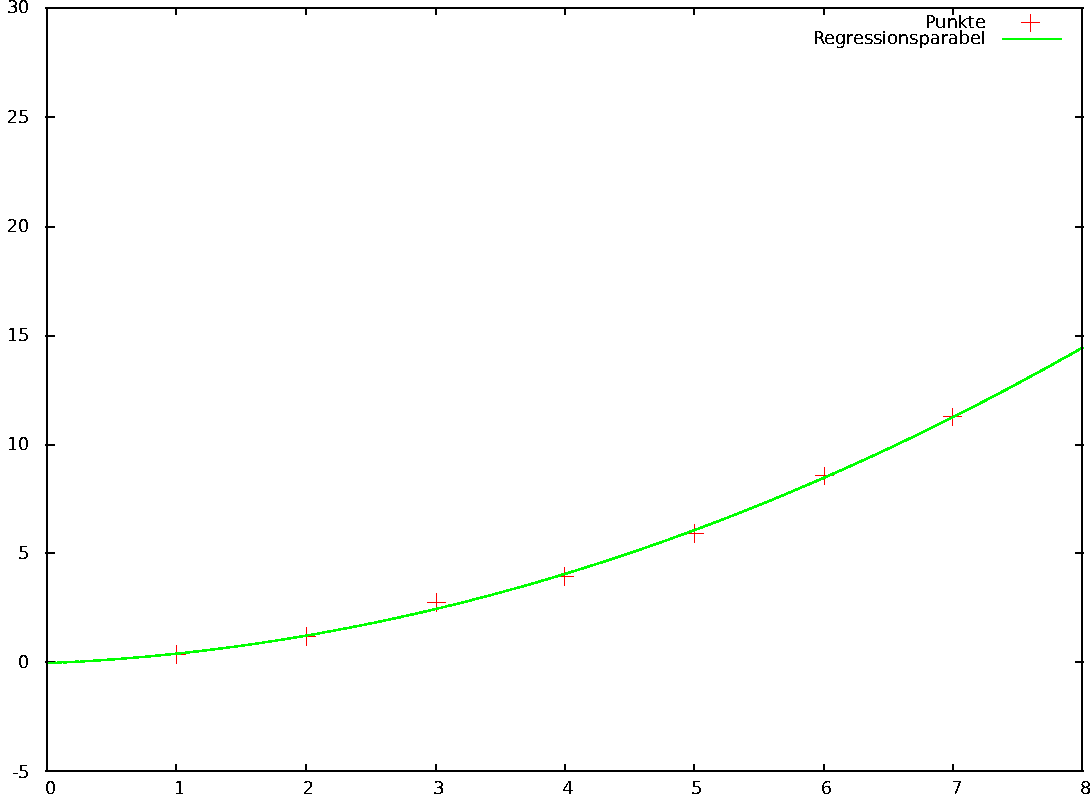
\includegraphics[scale=0.8]{img/quad_regression.pdf}
	\caption{Eine quadratische Regression mit 7 verschiedenen Punkten}
\end{figure}

\section{Korrelationskoeffizient}
\[ r_{xy} = \frac{\sigma_{xy}}{\sigma_x \cdot \sigma_y} = \frac{\mathlarger{\frac{1}{n}} \mathlarger{\sum_{i=1}^n} x_i \cdot y_i ~ - \overline{x}\cdot\overline{y}}{\sqrt{\mathlarger{\frac{1}{n}} \mathlarger{\sum_{i=1}^n} (x_i-\overline{x})^2} \cdot \sqrt{\mathlarger{\frac{1}{n}} \mathlarger{\sum_{i=1}^n} (y_i-\overline{y})^2}} \]

\part{2. Kantonsschule}
\chapter{Analytische Geometrie}

\section{Pfeile}
\subsection{Ortspfeile}
\section{Vektoren}
Vektoren sind die Menge aller Pfeile, die mit derselben Kraft in die selbe Richtung zeigen.

\[ \vec{a} = \left(\begin{array}{l}2\\3\end{array}\right) \]

\subsection{Vektoraddition}
Bei der Vektoraddition werden die beiden x-Komponenten, sowie die beiden y-Komponenten miteinander addiert.
\[ \left(\begin{array}{c}1\\3\end{array}\right) + \left(\begin{array}{c}2\\4\end{array}\right) = \left(\begin{array}{c}3\\7\end{array}\right) \]

\subsection{Vektorsubtraktion}
Die Vektorsubtraktion erfolgt analog zur Vektoraddition.
\[ \left(\begin{array}{c}3\\7\end{array}\right) - \left(\begin{array}{c}1\\3\end{array}\right) = \left(\begin{array}{c}2\\4\end{array}\right) \]

\subsection{Skalarmultiplikation}
Die Multiplikation zweier Vektoren ergibt ein Skalar.
\[ \left(\begin{array}{c}1\\3\end{array}\right) \cdot \left(\begin{array}{c}2\\4\end{array}\right) = 1 \cdot 2 + 3 \cdot 4 =  14\]

\subsection{Länge eines Vektores}
Der Betrag des Vektors entspricht der Länge des Vektors auf der Ebene.
\[ \left\vert\left(\begin{array}{c}1\\3\end{array}\right)\right\vert = \sqrt{1^2 + 3^2} = \sqrt{10}\]

\subsection{Berechnungen in der Geometrie}
Berechne den fehlenden Punkt $D$ des Parallelogrammes.
\begin{figure}[h]
	\centering
	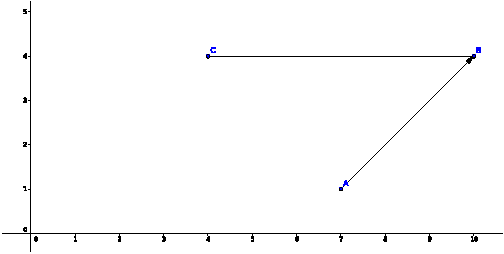
\includegraphics[scale=2]{img/vektor_parallelogramm.pdf}
	\caption{Ein Parallelogramm, dessen Punkt $D$ über den Vektor $AB$  berechnet werden kann}
\end{figure}\\
Zuerst muss der Vektor $\overrightarrow{AB}$ umgekehrt werden, das heisst, x- und y-Komponente wechseln das Vorzeichen.
\[ \vec{a} = \left(\begin{array}{c} 3\\ 3 \end{array}\right); \quad\quad  -\vec{a} = \left(\begin{array}{c} -3\\ -3 \end{array}\right)\]
Nun addiert man den Vektor $-\vec{a}$ zum Ortspfeil $\vec{C}$, dann erhält man den Ortspfeil $\vec{D}$.
\[ \left(\begin{array}{c}4\\4\end{array}\right) + \left(\begin{array}{c}-3\\-3\end{array}\right) = \left(\begin{array}{c}1\\1\end{array}\right) \]
Folglich ist der Punkt $D = (1 \vert 1)$.

\subsection{Kippregeln}
Vektoren lassen sich nach links oder rechts um $90^{\circ}$ kippen.
Die gekippten Vektoren berechnen sich wie folgt:
\[ \vec{a} = \left(\begin{array}{c} 5\\ 2 \end{array}\right); \quad\quad \vec{a}_l = \left(\begin{array}{c} -2\\ 5 \end{array}\right); \quad\quad \vec{a}_r = \left(\begin{array}{c} 2\\ -5 \end{array}\right); \]
\begin{figure}
\centering
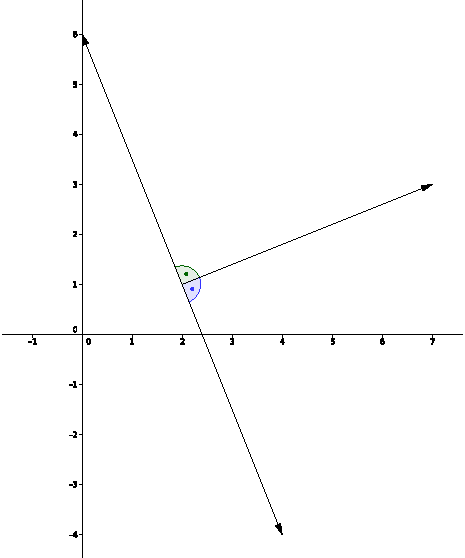
\includegraphics[scale=1]{img/vektor_kippen.pdf}
\caption{Gekippte Vektoren}
\end{figure}

\subsection{Orthogonalitätskriterium}
Zwei Vektoren gelten als zueinander orthogonal, wenn ihr skalares Produkt 0 ist.
\[ \vec{a} \perp \vec{b} \Longleftrightarrow \vec{a} \cdot \vec{b} = 0 \]

\subsection{VP Formel}

\subsection{VW Formel}

\part{Anhang}
\listoffigures

\end{document}
